   
\begin{itemize}
\item Le \textbf{cube} est un prisme droit à base carrée et dont la hauteur est égale à la longueur de l'arête du carré de base.

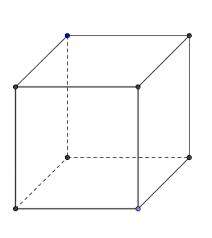
\includegraphics[scale=0.3]{RepS-cube.jpg} 

\item Un \textbf{pavé droit} est un prisme droit à base rectangulaire. L'autre du nom du pavé droit est le \textbf{parallélépipède rectangle}.

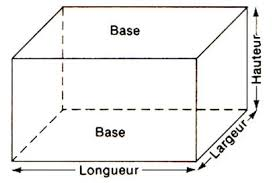
\includegraphics[scale=0.3]{RepS-pave.jpg} 

\item Il existe des prismes droits à base pentagonale, hexagonale, \ldots{}

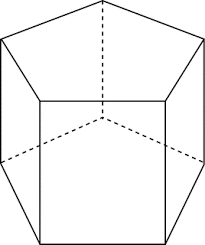
\includegraphics[scale=0.3]{RepS-pentagonale.png} 
\hspace*{1cm}
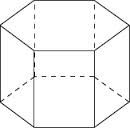
\includegraphics[scale=0.6]{RepS-prisme_hexagonale.jpg}
\hspace*{0.5cm} 
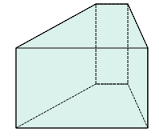
\includegraphics[scale=0.6]{RepS-pirsme_quelconque.png} 
\end{itemize}